\documentclass[final,hyperref={pdfpagelabels=false}]{beamer}
\usepackage{grffile}
\mode<presentation>{\usetheme{I6pd2}}{
% \usetheme{Berlin}
\usetheme{Dreuw}
}
\usepackage[english]{babel}
\usepackage[latin1]{inputenc}
\usepackage{amsmath,amsthm, amssymb, latexsym}
%\usepackage{times}\usefonttheme{professionalfonts}  % obsolete
%\usefonttheme[onlymath]{serif}
\boldmath
\usepackage[orientation=portrait,size=a0,scale=1.4,debug]{beamerposter}


    
\usepackage{multicol}
\usepackage{tikz,pgfplots}
\usepackage{pgfplotstable}




% change list indention level
% \setdefaultleftmargin{3em}{}{}{}{}{}


%\usepackage{snapshot} % will write a .dep file with all dependencies, allows for easy bundling


\usepackage{array,booktabs,tabularx}
\newcolumntype{Z}{>{\centering\arraybackslash}X} % centered tabularx columns
\newcommand{\pphantom}{\textcolor{ta3aluminium}} % phantom introduces a vertical space in p formatted table columns??!!

\listfiles

%%%%%%%%%%%%%%%%%%%%%%%%%%%%%%%%%%%%%%%%%%%%%%%%%%%%%%%%%%%%%%%%%%%%%%%%%%%%%%%%%%%%%%
\graphicspath{{figures/}}
 
\title{\huge Fusion Moves for Correlation Clustering}
\author{Thorsten Beier, Fred A. Hamprecht and J\"org H. Kappes }
\institute[RWTH Aachen University]{Heidelberg Collaboratory for Image Processing, University of Heidelberg, Germany}
\date[\today]{\today}

%%%%%%%%%%%%%%%%%%%%%%%%%%%%%%%%%%%%%%%%%%%%%%%%%%%%%%%%%%%%%%%%%%%%%%%%%%%%%%%%%%%%%%
\newlength{\columnheight}
\setlength{\columnheight}{105cm}

\DeclareMathOperator*{\argmin}{arg\,min}
\DeclareMathOperator*{\argmax}{arg\,max}

%%%%%%%%%%%%%%%%%%%%%%%%%%%%%%%%%%%%%%%%%%%%%%%%%%%%%%%%%%%%%%%%%%%%%%%%%%%%%%%%%%%%%%
\begin{document}
\setbeamertemplate{bibliography item}{[\theenumiv]}
\begin{frame}
  \begin{columns}
    % ---------------------------------------------------------%
    % Set up a column 
    \begin{column}{.49\textwidth}
      \begin{beamercolorbox}[center,wd=\textwidth]{postercolumn}
        \begin{minipage}[T]{.95\textwidth}  % tweaks the width, makes a new \textwidth
          \parbox[t][\columnheight]{\textwidth}{ % must be some better way to set the the height, width and textwidth simultaneously
            % Since all columns are the same length, it is all nice and tidy.  You have to get the height empirically
            % ---------------------------------------------------------%
            % fill each column with content            
            \begin{block}{Introduction}

            \small  
            \begin{itemize}
                \item  Correlation clustering~\cite{Bansal-2002}, or multicut partitioning~\cite{chopra_1993_mp} ,
                is widely used partitioning an undirected graph with positive and negative edge weights
                ~\cite{andres_2011_iccv,kroeger_2012_eccv,yarkony_2012_eccv,alush_2013_simbad}. 
                \item NP-hard,  exact solvers do not scale and approximative solvers often give bad results.
                \item Inspired by \cite{Lempitsky-2010} we define fusion moves for the correlation clustering
                where we iteratively fuses the current and a proposed partitioning and monotonously improve the partitioning
                \item Scales well, gives near optimal solutions, has good anytime performance
            \end{itemize}

            % Correlation clustering~\cite{Bansal-2002}, or multicut partitioning~\cite{chopra_1993_mp} ,
            % is widely used partitioning an undirected graph with positive and negative edge weights
            % ~\cite{andres_2011_iccv,kroeger_2012_eccv,yarkony_2012_eccv,alush_2013_simbad}.
            % Since it is NP-hard, exact solvers do not scale and approximative solvers often give bad results.
            % Inspired by \cite{Lempitsky-2010} Here we define fusion moves for the correlation clustering problem.
            % Our algorithm iteratively fuses the current and a proposed partitioning which  monotonously improves
            % the partitioning. It scales well gives near optimal solutions, and has
            % a good anytime performance.
           
            \end{block}
            \vfill
            \begin{block}{Correlation Clustering / Multicut Objective:}
            \begin{small}
            \begin{itemize}
            \item Given a weighted graph $G=(V,E,w)$ 
            \item We consider the problem of segmenting $G$ such that the costs
            of the edges between distinct segments is minimized. 
            \item Can be formulated in the node domain
            by assigning each node $i$ a label $l_i \in \mathbb{N}$
            \begin{align}
              l^* &= \argmin_{l \in \mathbb{N}^{|V|}} \sum_{ (i,j) \in E } w_{ij} \cdot [l_{i} \neq l_{j}], \label{eq:nodeproblem}
            \end{align} 
            \item Can be formulated in in the edge domain, by labeling each edge $e$ as cut $y_e=1$ or uncut $y_e=0$ 
            \begin{align}
              y^* &= \argmin_{y \in P(G)} \sum_{ (i,j) \in E } w_{ij} \cdot y_{ij} \label{eq:edgeproblem}.%\\ 
            \end{align}
            \end{itemize}
            \centering
            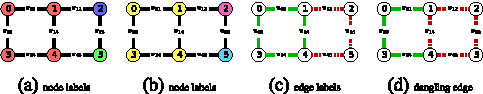
\includegraphics[width=0.9\linewidth]{ne-crop.pdf}
            \end{small}

            \end{block}



            \vfill
            \begin{block}{Correlation Clustering Fusion Moves}
              \begin{small}

              \begin{itemize}

              \item Given two proposal solutions $y'$ and $y''$, $E_0^{\breve{y}}$ is the set of edges
              which are uncut in $y'$ and $y''$.
              %
              \begin{align}
              \breve{y}_{ij}    & = \max\{ y_{ij}', y_{ij}''\}  & \forall {ij}\in E\\  % y' \cup y'' \\
              E_0^{\breve{y}}  & =  \{ ij \in E \; | \; \breve{y}_{ij} = 0 \}
              \end{align}
              %
              \item The fusion move for correlation clustering is solving Eq.~\ref{eq:edgeproblem}
              with additional \emph{must-link constraints} for all edges in $E_0^{\breve{y}}$.
              %
              \begin{align}
                y^* &= \argmin_{y \in P(G)} \sum_{ (i,j) \in E } w_{ij} \cdot y_{ij} \label{eq:fusion_move_a}.\\ 
                    &\quad \textrm{s.t.} \quad y_{ij} = 0 & \forall (i, j) \in E_0^{\breve{y}} \nonumber
              \end{align}
              %
              
              \item We can reformulate~\ref{eq:fusion_move_a}
              into a correlation clustering problem on a coarsened graph, where all nodes which are connected
              via must-link constraints are merged into single nodes.  We call this graph a \emph{contracted graph}.

              \item Any clustering $\bar{y}$ of the contracted graph $G_y=(V_y,E_y)$ can be \emph{back projected} to a clustering $\tilde{y}$ of the original graph $G=(V,E)$
              \end{itemize}
              \end{small}
              \vfill
              \vspace{2cm}
              \centering
              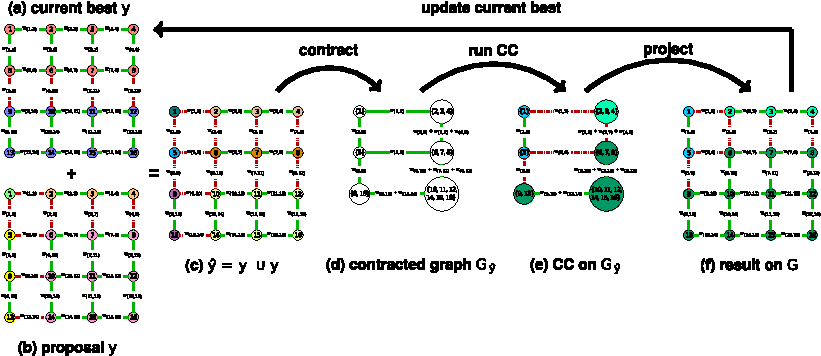
\includegraphics[width=1.0\linewidth]{si-crop.pdf}


            \end{block}
            \vfill
            \begin{block}{Proposal Generators}
            \begin{small}
            As discussed in~\cite{Lempitsky-2010}, proposals
            should have two properties: \emph{high quality} 
            and \emph{large diversity}.
            For correlation clustering fusion we add a third
            property: \emph{size}.  
            We use the following two proposal generators (see paper for details):
            \begin{itemize}
                \item \textbf{Randomized Hierarchical Clustering (RHC):}
                we add normally distributed noise  $\mathcal{N}(0, \sigma_{ehc})$ to each edge weight.
                In each step the edge with the highest weight is contracted.

                \item \textbf{Randomized Watersheds (RWS):}
                The edge weighted watershed algorithm~\cite{meyer_2013}
                with random seeds can be used to find
                cheap proposals.
            \end{itemize}
            \end{small}
            \end{block}

          }
        \end{minipage}
      \end{beamercolorbox}
    \end{column}
    % ---------------------------------------------------------%
    % end the column

    % ---------------------------------------------------------%
    % Set up a column 
    \begin{column}{.49\textwidth}
      \begin{beamercolorbox}[center,wd=\textwidth]{postercolumn}
        \begin{minipage}[T]{.95\textwidth} % tweaks the width, makes a new \textwidth
          \parbox[t][\columnheight]{\textwidth}{ % must be some better way to set the the height, width and textwidth simultaneously
            % Since all columns are the same length, it is all nice and tidy.  You have to get the height empirically
            % ---------------------------------------------------------%
            % fill each column with content
            
            \begin{block}{Results}
            \small{
            Among all proposed solvers, Fusion-HC-MC has the best overall anytime performance.
            }
            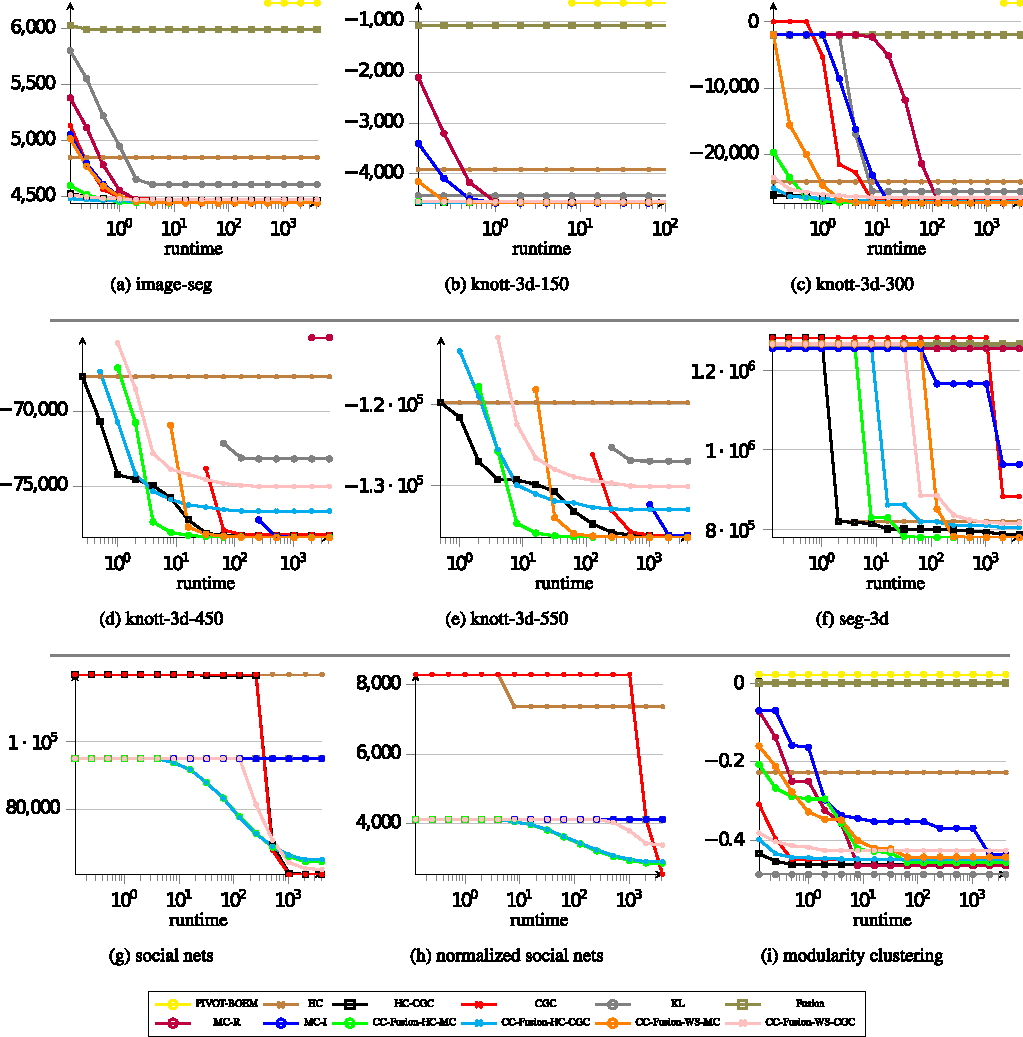
\includegraphics[width=0.9\linewidth]{res_images.pdf}


            \end{block}
            \vfill
            \begin{block}{Evaluation by Segmentation Metrics}
                \small{
                Evaluation by Variation of Information (VOI) and
                Rand Index (RI) for datasets with available ground truth:
                }
                \vspace{1cm}


              \centering
              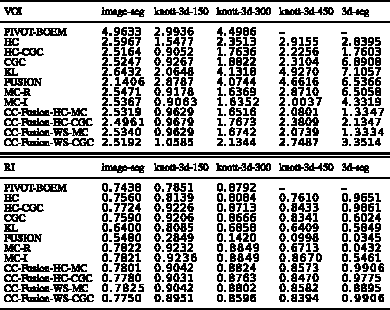
\includegraphics[width=0.7\linewidth]{virib.pdf}            
            \end{block}
            \vfill
            % \begin{block}{Cofonclusions}
            %     We have presented a fast and scalable 
            %     approximate solver for correlation 
            %     clustering, named Correlation Clustering Fusion (CC-Fusion).
            %     It is orthogonal to previous research, \ie it can be combined with
            %     any correlation clustering solver.
            %     %
            %     The best solution is iteratively improved 
            %     by a fusion with proposal solutions.
            %     The fusion move itself is formulated as correlation
            %     clustering on a smaller graph with fewer edges and nodes
            %     and can therefore be solved much faster than the original problem.
            %     %
            %     Our evaluation shows that several CC-Fusion algorithms
            %     outperform state-of-the-art solvers w.r.t. anytime performance 
            %     with increasing problem size.
            % \end{block}
            \vfill
            \begin{block}{References}
                \begin{multicols}{2}
                \footnotesize
                \bibliographystyle{ieee}
                \bibliography{egbib}
                \end{multicols}
            \end{block}
            \vfill
          }
          % ---------------------------------------------------------%
          % end the column
        \end{minipage}
      \end{beamercolorbox}
    \end{column}
    % ---------------------------------------------------------%
    % end the column
  \end{columns}
  \vskip1ex
  %\tiny\hfill\textcolor{ta2gray}{Created with \LaTeX \texttt{beamerposter}  \url{http://www-i6.informatik.rwth-aachen.de/~dreuw/latexbeamerposter.php}}
  %\tiny\hfill{Created with \LaTeX \texttt{beamerposter}  \url{http://www-i6.informatik.rwth-aachen.de/~dreuw/latexbeamerposter.php} \hskip1em}
\end{frame}
\end{document}


%%%%%%%%%%%%%%%%%%%%%%%%%%%%%%%%%%%%%%%%%%%%%%%%%%%%%%%%%%%%%%%%%%%%%%%%%%%%%%%%%%%%%%%%%%%%%%%%%%%%
%%% Local Variables: 
%%% mode: latex
%%% TeX-PDF-mode: t
%%% End:
